\appendix
\pagenumbering{Roman}

\chapter{Appendix}


 \section{Supplemental Figures}

  \begin{figure}[!ht]
   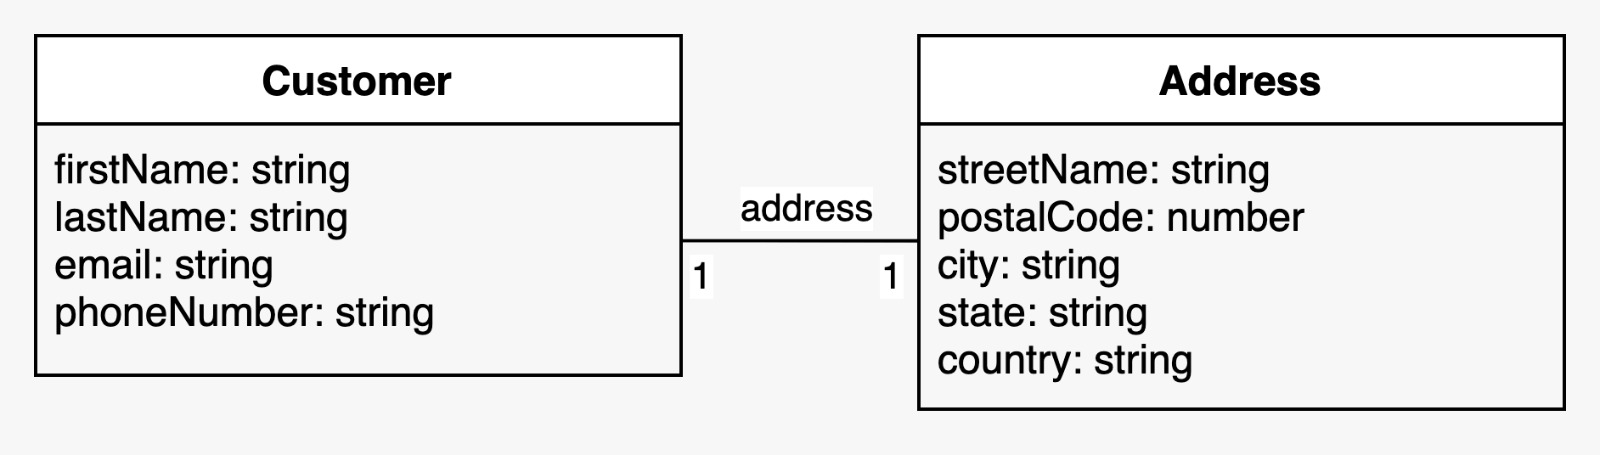
\includegraphics[width=\textwidth]{diagrams/entity_customer.jpeg}
   \caption{UML diagram of the customer model}
   \label{fig:customer_uml}
  \end{figure}
  
  \begin{figure}[!ht]
    \centering
    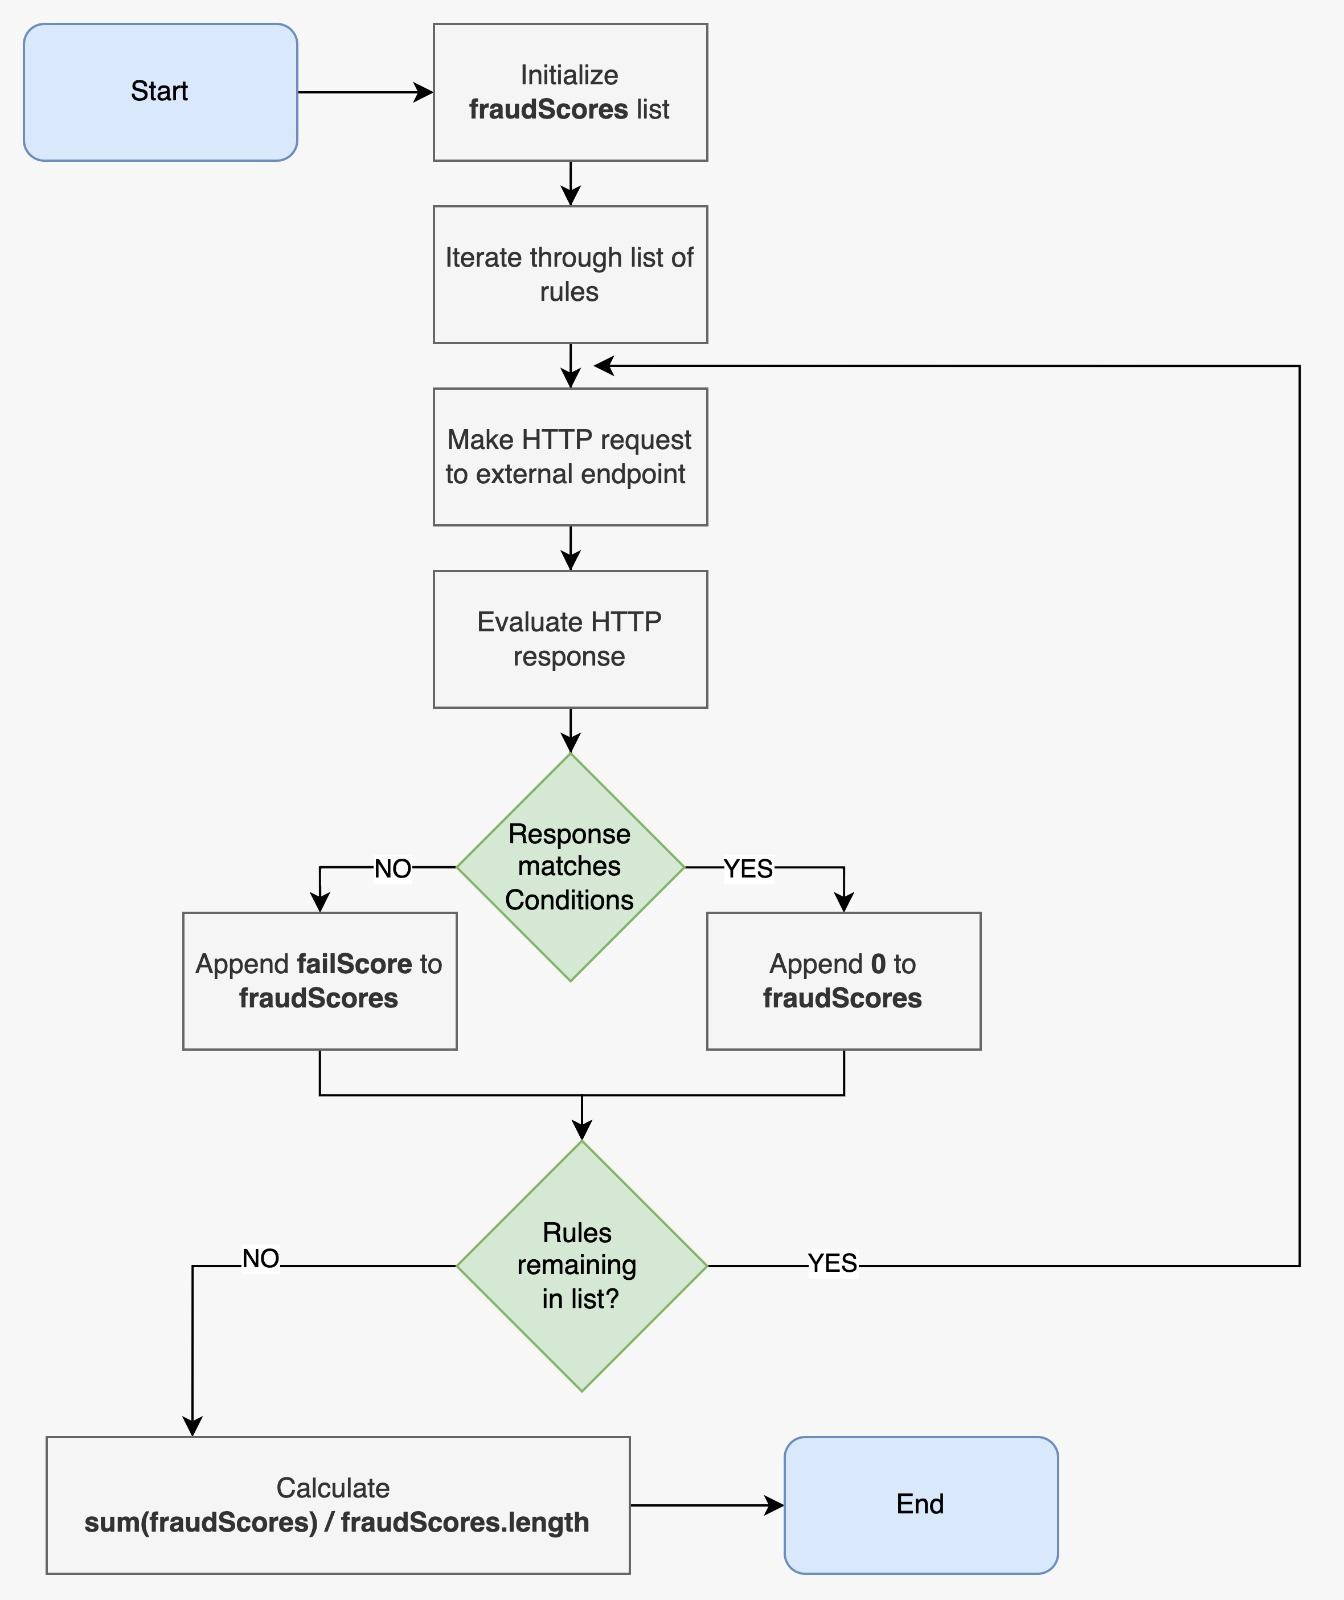
\includegraphics[width=0.8\textwidth]{diagrams/flow_validation_process.jpeg}
    \caption{Flow diagram of a validation process}
    \label{fig:flow_validation}
  \end{figure}

 \section{Supplemental Source Codes}
 
  \begin{lstlisting}[caption={\emph{Prisma} schema of a validation rule (Prisma)}, label={code:prisma}]
 model ValidationRule {
   id                  String    @id @default(auto()) @map("_id") @db.ObjectId
   name                String    @unique
   skip                Boolean
   priority            Int
   endpoint            String
   method              String
   failScore           Float
   condition           Json
   retryStrategy       Json?
   requestUrlParameter Json?
   requestBody         Json?
   requestHeader       Json?
 }
  \end{lstlisting}

\section{Quell-Code}

\section{Tipps zum Schreiben Ihrer Abschlussarbeit}

\begin{itemize}
\item Achten Sie auf eine neutrale, fachliche Sprache. Keine \glqq{}Ich\grqq{}-Form.
\item Zitieren Sie zitierf\"ahige und -w\"urdige Quellen (z.B. wissenschaftliche Artikel und Fachb\"ucher; nach M\"oglichkeit keine Blogs und keinesfalls Wikipedia\footnote{Wikipedia selbst empfiehlt, von der Zitation von Wikipedia-Inhalten im akademischen Umfeld Abstand zu nehmen.}). 
\item Zitieren Sie korrekt und homogen.
\item Verwenden Sie keine Fu{\ss}noten f\"ur die Literaturangaben.
\item Recherchieren Sie ausf\"uhrlich den Stand der Wissenschaft und Technik.
\item Achten Sie auf die Qualit\"at der Ausarbeitung (z.B. auf Rechtschreibung).
\item Informieren Sie sich ggf. vorab dar\"uber, wie man wissenschaftlich arbeitet bzw. schreibt:
\begin{itemize}
\item Mittels Fachliteratur\footnote{Z.B.}, oder
\item Beim Lernzentrum\footnote{Weitere Informationen zum Schreibcoaching finden sich hier: \url{https://www.htw-berlin.de/studium/lernzentrum/studierende/schreibcoaching/}; letzter Zugriff: 13 VI 19.}.
\end{itemize}
\item Nutzen Sie \LaTeX\footnote{Kein Support bei Installation, Nutzung und Anpassung allf\"alliger \LaTeX-Templates!}.
\end{itemize}



\newpage
% Letzte Seite
\thispagestyle{empty}      
\noindent

\newpage
\section*{Eidesstattliche Versicherung}
Hiermit versichere ich an Eides statt durch meine Unterschrift, dass ich die vorstehende Arbeit selbstst\"andig und ohne fremde Hilfe angefertigt und alle Stellen, die ich w\"ortlich oder ann\"ahernd w\"ortlich aus Ver\"offentlichungen entnommen habe, als solche kenntlich gemacht habe, mich auch keiner anderen als der angegebenen Literatur oder sonstiger Hilfsmittel bedient habe. Die Arbeit hat in dieser oder \"ahnlicher Form noch keiner anderen Pr\"ufungsbeh\"orde vorgelegen.\\
\linebreak[4]
\linebreak[4]
\linebreak[4]
\linebreak[4]
-------------------------------------------------------\linebreak[4]
22.07.2022, Berlin

